\chapter{Studiu de piață / Soluții existente}
\label{chapter:studiuPiata}

\section{Alte soluții existente}
\label{sec:proj}
\subsection{Colorado Edu}

Prima soluție analizată este Colorado Edu, o platofrmă care oferă acoperire pe multiple materii după cum se poate observa în captura
următoare.

\fig[width=1\textwidth]{imgs/phet.png}{fig:distributie_persoane}{Captură de ecran de pe soluția Phet Colorado Edu}

Se poate observa designul simplu și intuitiv și suportul relativ extins pe materii. Are și o interactivitate bună la nivel de simulări și alt 
avantaj e că are acces gratuit. Totuși, nu are un sistem de evaluare integrat și nu permite crearea de teste personalizate. De asemenea, nu are
un sistem de management al utilizatorilor, ceea ce face ca utilizarea platformei să fie limitată la simulări ad-hoc, iar ținta principală ca științelor
curiculum este SUA și nu România.

\subsection{invatamate.com}


\fig[width=1\textwidth]{imgs/invatamate.png}{fig:invatamate}{Captură de ecran de pe platforma invatamate.com}

Cea de-a doua soluție analizată este invatamate.com, o platformă care oferă o suită de cursuri, vizualizări și simulări online.
După cum se poate observa în captura de ecran, platforma are un design relativ învechit și nu foarte atractiv, dar
conține multiple resurse utile. Deși numele sugerează că platforma este dedicată matematicii, ea are și simulări de astronomie
și joculețe interactive mai generale.


Problema este iar că nu are un sistem de management al utilizatorilor și nici suport pentru evaluare integrat.
Lipsa acestor funcționalități face ca platforma să nu fie foarte utilă în mediul educațional, iar utilizarea ei să fie limitată 
la joculețe simple și triviale. Alte limitări ale platformei sunt că folosește Flash pentru majoritate jocurilor științelor
chiar integrări cu Kahoot pentru unele, iar resursele sunt de asemenea legate din surse externe în unele cazuri.
De asemeea, experiența nu este cea mai modernă, intuitivă și placută după cum se poate vedea în capturile următoare.

\newpage
\begin{figure}[htb]
    \centering
    \begin{minipage}[b]{0.49\textwidth}
        \centering
        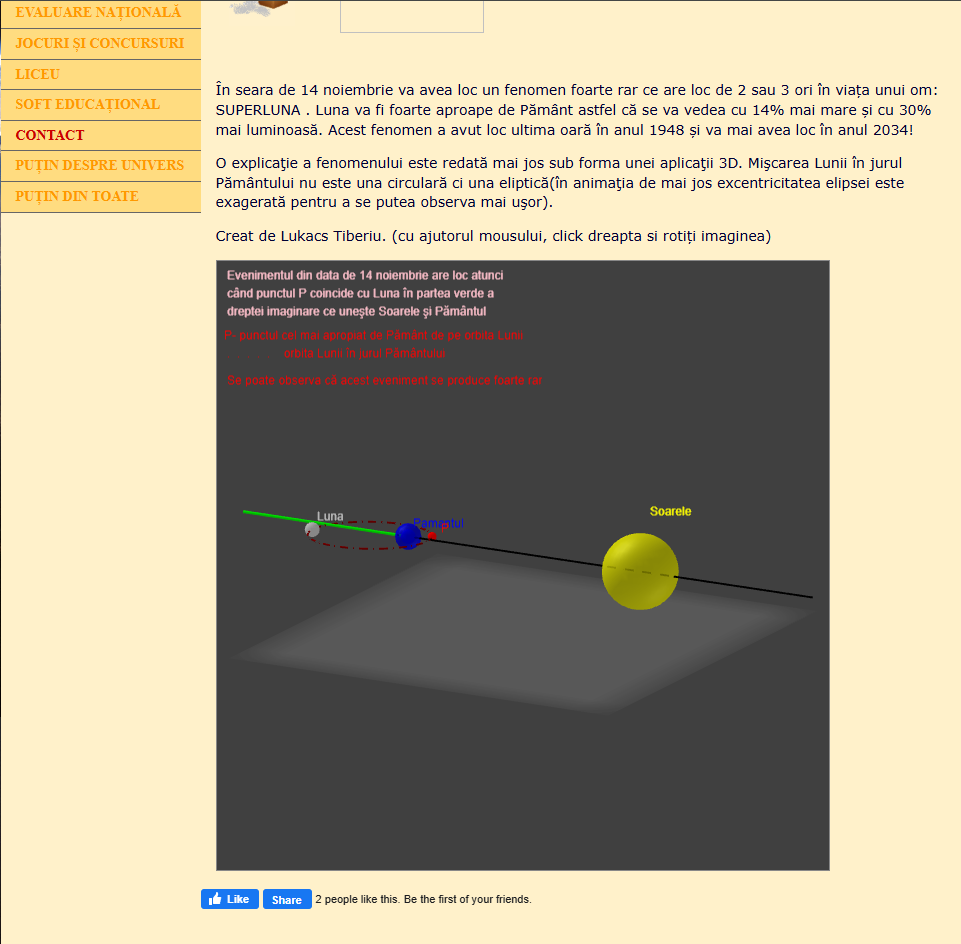
\includegraphics[width=\textwidth]{imgs/invatamatesimulare.png}
        \caption{Simulări de pe platforma invatamate.com}
        \label{fig:invatamatesimulare}
    \end{minipage}
    \hfill
    \begin{minipage}[b]{0.49\textwidth}
        \centering
        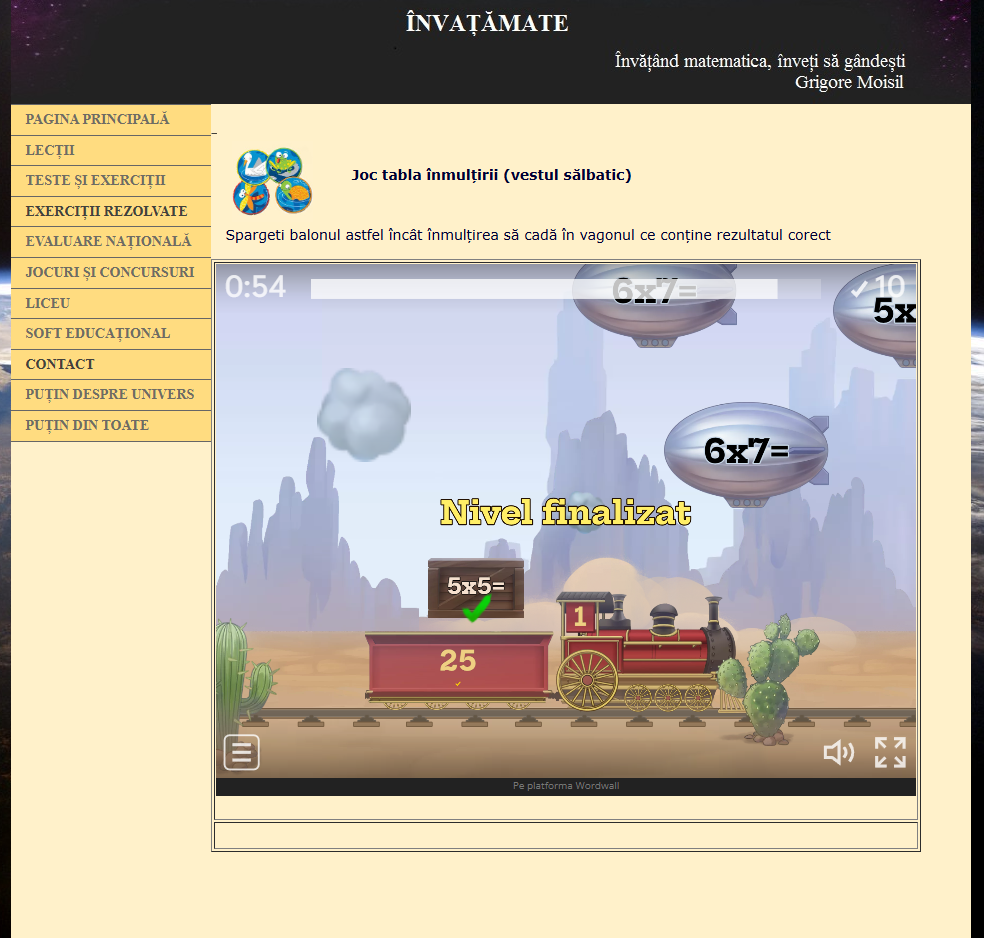
\includegraphics[width=\textwidth]{imgs/invatamatejoc.png}
        \caption{Jocuri de pe platforma invatamate.com}
        \label{fig:invatamatesjoc}
    \end{minipage}
\end{figure}


\subsection{Mozaweb.com}

Această soluție are o arhitectură cu produse pentru mai multe roluri (pentru elevi, pentru profesori, pentru școli) și o experiență de utilizare
plăcută și intuitivă. Se poate observa în captura de ecran de mai jos cum arată interfața de întâmpinare a utilizatorului.

\fig[width=0.8\textwidth]{imgs/mozaweb.png}{fig:mozaweb}{Captură de ecran de pe platforma mozaweb.com}

Se poate observa suportul pentru numeroase materii și din zona STEM, dar și pentru alte domenii. De asemenea, platforma are simulări foarte
profesioniste și interactive, dar dezavantajele mari sunt prețurile abonametelor pentru că discutăm de o platformă comercială și nu gratuită.
De asemenea pentru simulări este necesar să se instaleze un plugin extern, reducând astfel accesibilitatea platformei. Se poate observa mai jos
gama de simulări și necesitatea plugin-ului.

\fig[width=1\textwidth]{imgs/mozawebplugin.png}{fig:mozaweb}{Simulări și dovada plugin-ului necesar pentru a le rula}

Ținta aceste platforme este una comercială mai mult decât educațională, iar prețurile sunt relativ mari pentru toate tipurile de utilizatori.


\subsection{iqboard.ro}

Ultima soluție analizată este iqboard.ro, o platformă care oferă o suită de resurse educaționale în limba română, cu multiple moduri 
de lucru, multi touch, bazat pe un sistem de abonamente. Are o interfață interesantă și atractivă și suport extins educațional după cum se poate observa
în captura de ecran de mai jos (figura \ref{fig:iqboard}). 

Dezavantajele majore sunt prețurile extrem de mari pentru utilizatori (la nivel de sute de euro după cum se poate observa în figura \ref{fig:iqboard}).
Prețul este relativ nejustificat deși materialele sunt de calitate bună și platforma are un design interactiv și atractiv.
în figura \ref{fig:iqboardsimulari} se poate urmări un exemplu de simulare disponibilă pe platformă. Platforma are moduri separate pentru 
pregătire, predare și mod desktop, dar nu are un sistem de management al utilizatorilor sau vreun sistem de evaluare sau 
urmărire a progresului utilizatorilor.

Ca alte funcționalități, platforma se laudă cu modul multi-user care poate fi folosit in modul tabla sau full-screen.
Dupa selectarea instrumentului dorit, utilizatorii pot lucra simultan pe tabla, cu modul multi-screens (modul petrecere), 
cu posibilitate de folosire simultana a doua table interactive (modul MX2) și cu modul raspuns interactiv.

\begin{figure}[htb]
    \centering
    \begin{minipage}[b]{0.49\textwidth}
        \centering
        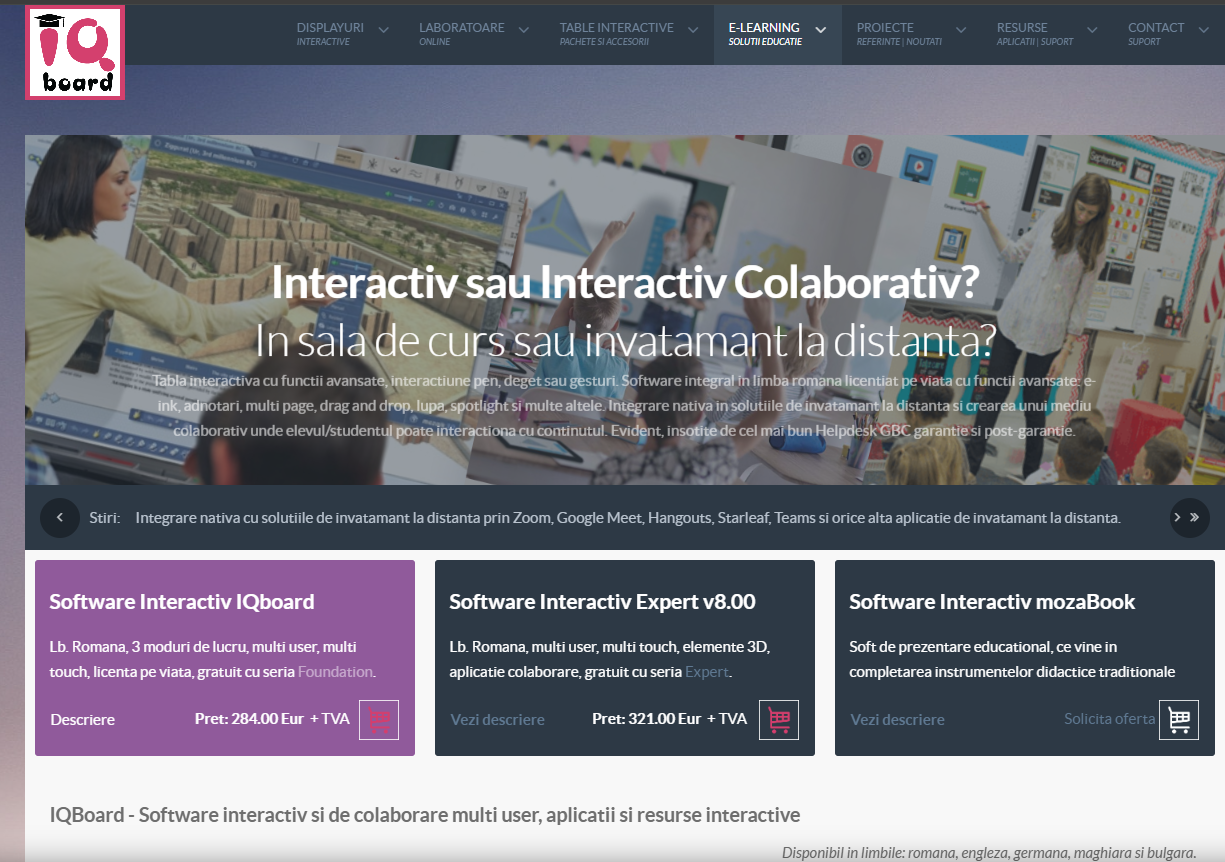
\includegraphics[width=\textwidth]{imgs/iqboard.png}
        \caption{Captură de ecran de pe platforma iqboard.ro}
        \label{fig:iqboard}
    \end{minipage}
    \hfill
    \begin{minipage}[b]{0.49\textwidth}
        \centering
        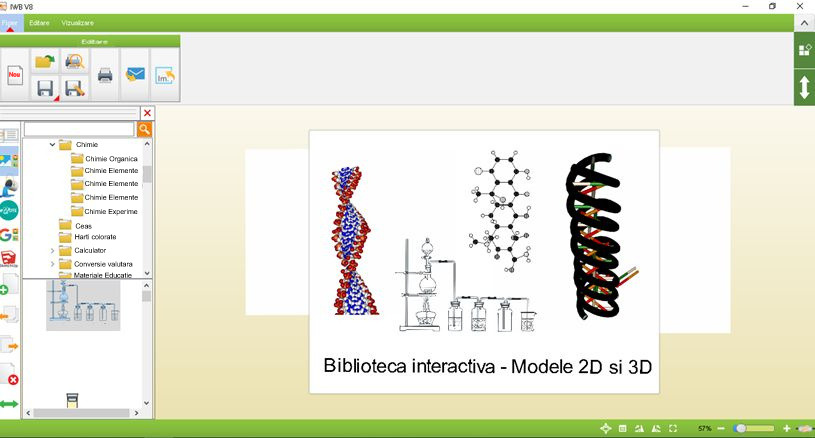
\includegraphics[width=\textwidth]{imgs/iqboardsimulari.jpg}
        \caption{Simulări de pe platforma iqboard.ro}
        \label{fig:iqboardsimulari}
    \end{minipage}
\end{figure}


\section{Raportarea la alte soluții}
\label{sub-sec:proj-scope}


\begin{itemize}
    \item \textbf{O singură platformă completă pentru toate materiile STEM}
    În timp ce Phet sau Invatamate se concentrează mai mult pe un subiect, VisioScience3D
    va oferi un mediu unificat cu module interactive de matematică, fizică, chimie, informatică și
    chiar astronomie, reducând necesitatea schimbării constante de aplicații.
    \item \textbf{Simulări 3D real-time și configurabile}
    Mozaweb de exemplu are mult suport pentru scene 3D, dar ele sunt predefinite şi nu pot fi adaptate dinamic. 
    VisioScience3D permite ajustarea parametrilor în timp real (forțe, unghiuri, constante) și animarea vectorilor.
    \item \textbf{Dashboard de monitorizare a progresului}
    Lipsa de raportare în timp real este o problemă la majoritatea soluţiilor gratuite. 
    Profesorii pot vizualiza instantaneu statistici legate de scoruri, dificultăţi întâmpinate și 
    pot adapta testele în funcție de nevoile elevilor.
    \item \textbf{Gamificare}
    Majoritatea platformelor nu au un sistem de gamificare bine definit. VisioScience3D va include elemente
    de gamificare pentru a spori implicarea elevilor.
\end{itemize}

\section{Motivația alegerii VisioScience3D de către utilizatori}
\label{sub-sec:proj-motivatie}

VisioScience3D răspunde foarte bine nevoilor profesorilor și elevilor de azi.
Oferă simultan simulări 3D real-time pentru toate disciplinele STEM, configurabile 
direct în browser în platformă, fără pluginuri externe. În timp ce multe platforme 
existente fie acoperă doar un număr limitat de subiecte, fie implică licențe costisitoare
sau dependențe externe (Mozaweb, IQBoard). VisioScience3D pune la dispoziție un mediu unic,
adaptat programei românești. Profesorii pot monitoriza progresul elevilor prin dashboard-uri
integrate și primesc rapoarte detaliate. Prin modelul gratis și nivelul simulărilor suportate,
VisioScience3D este un ecosistem complet, flexibil și orientat spre rezultatele elevilor.